\chapter{Simulación Circuital en LTspice}
\label{chap:simulacion}

Con el objeto de validar el diseño analítico y contrastar el comportamiento del amplificador bajo condiciones ideales
y comerciales, se realizaron simulaciones circuitales en el entorno LTspice. Se estudió el punto de polarización en
continua (.op) y la respuesta dinámica en el dominio del tiempo (.tran) para ambos casos.

\section{Directivas de Simulación y Modelos Empleados}

Para simular con fidelidad el transistor bipolar utilizado en laboratorio, se incorporó el modelo SPICE del BC546/BC547
con ganancia de corriente forward $B_f = 290$, valor concordante con los $\beta = 284$ medidos con el multímetro.

En el listado~\ref{list:directivas_spice} se presentan las directivas de simulación configuradas en el archivo esquemático.

\begin{lstlisting}[style=ltspice, caption={Directivas de simulación y modelo de transistor en LTspice.}, label={list:directivas_spice}]
* Modelo SPICE de transistor NPN (Philips) con Bf=290
.model BC546C NPN(Is=21.43f Xti=3 Eg=1.11 Vaf=74.03 Bf=290
+ Ise=43.11f Ne=1.442 Ikf=97.09m Nk=.5 Xtb=1.5 Br=9.837
+ Isc=144.3f Nc=1.522 Ikr=2.476 Rc=1 Cjc=5.25p Mjc=.3147
+ Vjc=.5697 Fc=.5 Cje=11.5p Mje=.6115 Vje=.8194 Tr=10n
+ Tf=443.2p Itf=.7 Vtf=4 Xtf=4 Vceo=65 Icrating=100m)

* Fuente de senal senoidal de entrada: Amplitud 10 mVp, f = 1 kHz
VBB n002 0 SINE(0 10m 1k)

* Directiva de analisis transitorio: inicio de guardado en 990 ms
.tran 0 1 990m
\end{lstlisting}

La directiva \lstinline[style=ltspice]{.tran 0 1 990m} ejecuta un análisis temporal durante un intervalo total de $1\s$,
pero comienza a almacenar los datos únicamente a partir de los $990\ms$. Esta decisión metodológica permite descartar
por completo el transitorio inicial de carga de los capacitores de acoplo ($C_1, C_2$) y desacoplo ($C_E$), registrando
exclusivamente el régimen permanente periódico correspondiente a los últimos diez ciclos de la señal a $1\kHz$.

\section{Simulación con Valores Teóricos Ideales}

En la figura~\ref{fig:sch_teorico} se presenta el esquema circuital implementado en LTspice con los resistores
teóricos calculados ($R_1 = 6.14\kohm$, $R_2 = 34.9\kohm$, $R_C = 1.2\kohm$, $R_E = 180\ohm$ y $R_L = 1\kohm$).

\begin{figure}[!ht]
  \centering
  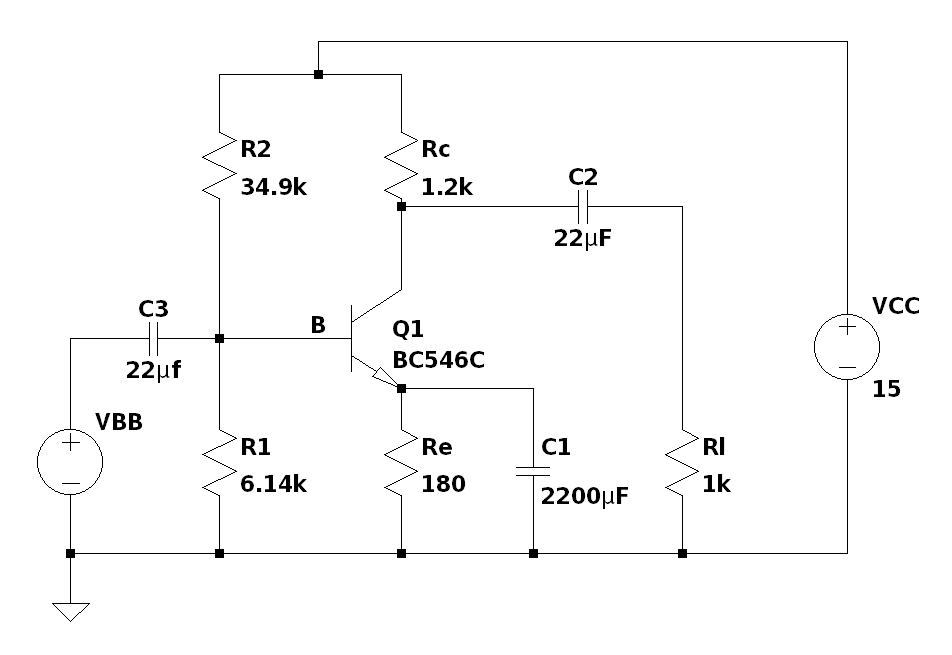
\includegraphics[width=0.82\textwidth]{images/ValoresTeoricos.png}
  \caption{Esquemático de simulación en LTspice con valores teóricos ideales de polarización.}
  \label{fig:sch_teorico}
\end{figure}

El cálculo del punto de operación en continua (.op) arrojó los siguientes valores de polarización:
\begin{itemize}
  \item Tensión de base: $V_B = 2.010\V$.
  \item Tensión de emisor: $V_E = 1.390\V$.
  \item Tensión de colector: $V_C = 5.772\V$.
  \item Tensión colector-emisor: $V_{CEQ} = V_C - V_E = 4.382\V$.
  \item Corriente de colector: $I_{CQ} = 7.690\mA$.
  \item Corriente de base: $I_{BQ} = 31.7\uA$.
\end{itemize}

Estos resultados se encuentran en concordancia con el diseño analítico de MES ($I_{CQ} = 7.79\mA$, $V_{CEQ} = 4.25\V$),
presentando una discrepancia de apenas $-1.28\%$ en corriente y $+3.11\%$ en tensión, atribuible a la caída de
tensión interna base-emisor del modelo SPICE ($V_{BE} = 0.620\V$) y al efecto Early modelado ($V_{af} = 74.03\V$).

\section{Simulación con Valores Normalizados Comerciales}

Posteriormente se simuló el circuito sustituyendo los valores teóricos por los resistores comerciales normalizados
seleccionados ($R_1 = 6.8\kohm$ y $R_2 = 39\kohm$). El esquemático correspondiente se exhibe en la figura~\ref{fig:sch_comercial}.

\begin{figure}[!ht]
  \centering
  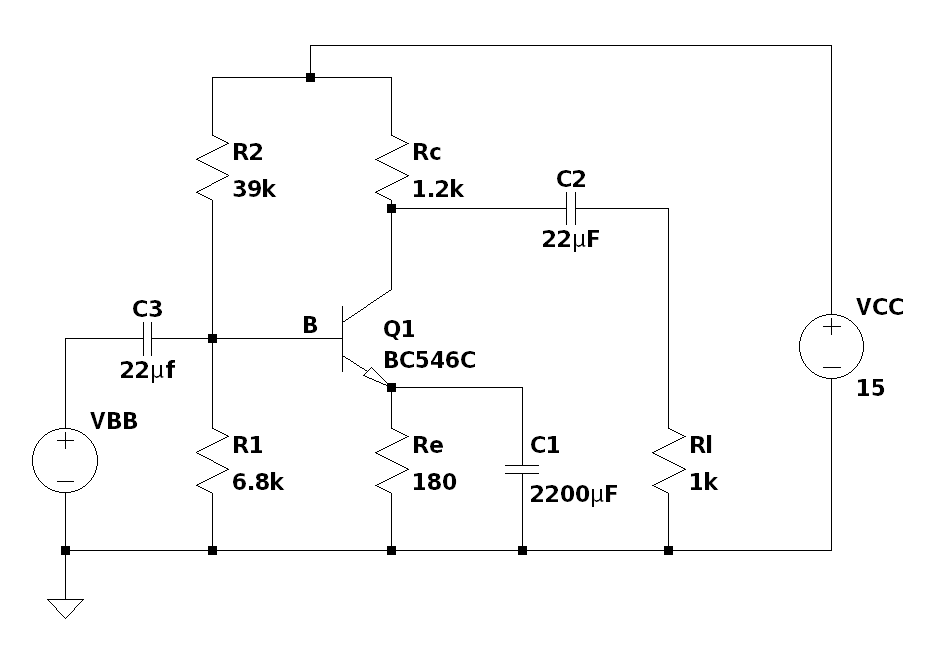
\includegraphics[width=0.82\textwidth]{images/ValoresComerciales.png}
  \caption{Esquemático de simulación en LTspice con valores comerciales normalizados.}
  \label{fig:sch_comercial}
\end{figure}

El punto de operación en continua con valores comerciales resultó:
\begin{itemize}
  \item Tensión de base: $V_B = 2.006\V$.
  \item Tensión de emisor: $V_E = 1.360\V$.
  \item Tensión de colector: $V_C = 5.970\V$.
  \item Tensión colector-emisor: $V_{CEQ} = 4.610\V$.
  \item Corriente de colector: $I_{CQ} = 7.525\mA$.
  \item Corriente de base: $I_{BQ} = 30.9\uA$.
\end{itemize}

Comparando con el cálculo analítico normalizado del capítulo~\ref{chap:normalizacion} ($I_{CQ} = 7.60\mA$,
$V_{CEQ} = 4.51\V$), la coincidencia es notable, con un error inferior al $1.0\%$ en corriente y del $2.2\%$ en tensión.

\section{Análisis de Formas de Onda y Ganancia Dinámica}

A partir de los archivos de exportación numérica de simulación (\texttt{ValoresTeoricos.txt} y
\texttt{ValoresComerciales.txt}), se procesaron los datos temporales del último período en régimen permanente.
En la figura~\ref{fig:sim_waveforms} se presentan las señales superpuestas de entrada ($v_{in}$) y salida ($v_o$).

\begin{figure}[!ht]
  \centering
  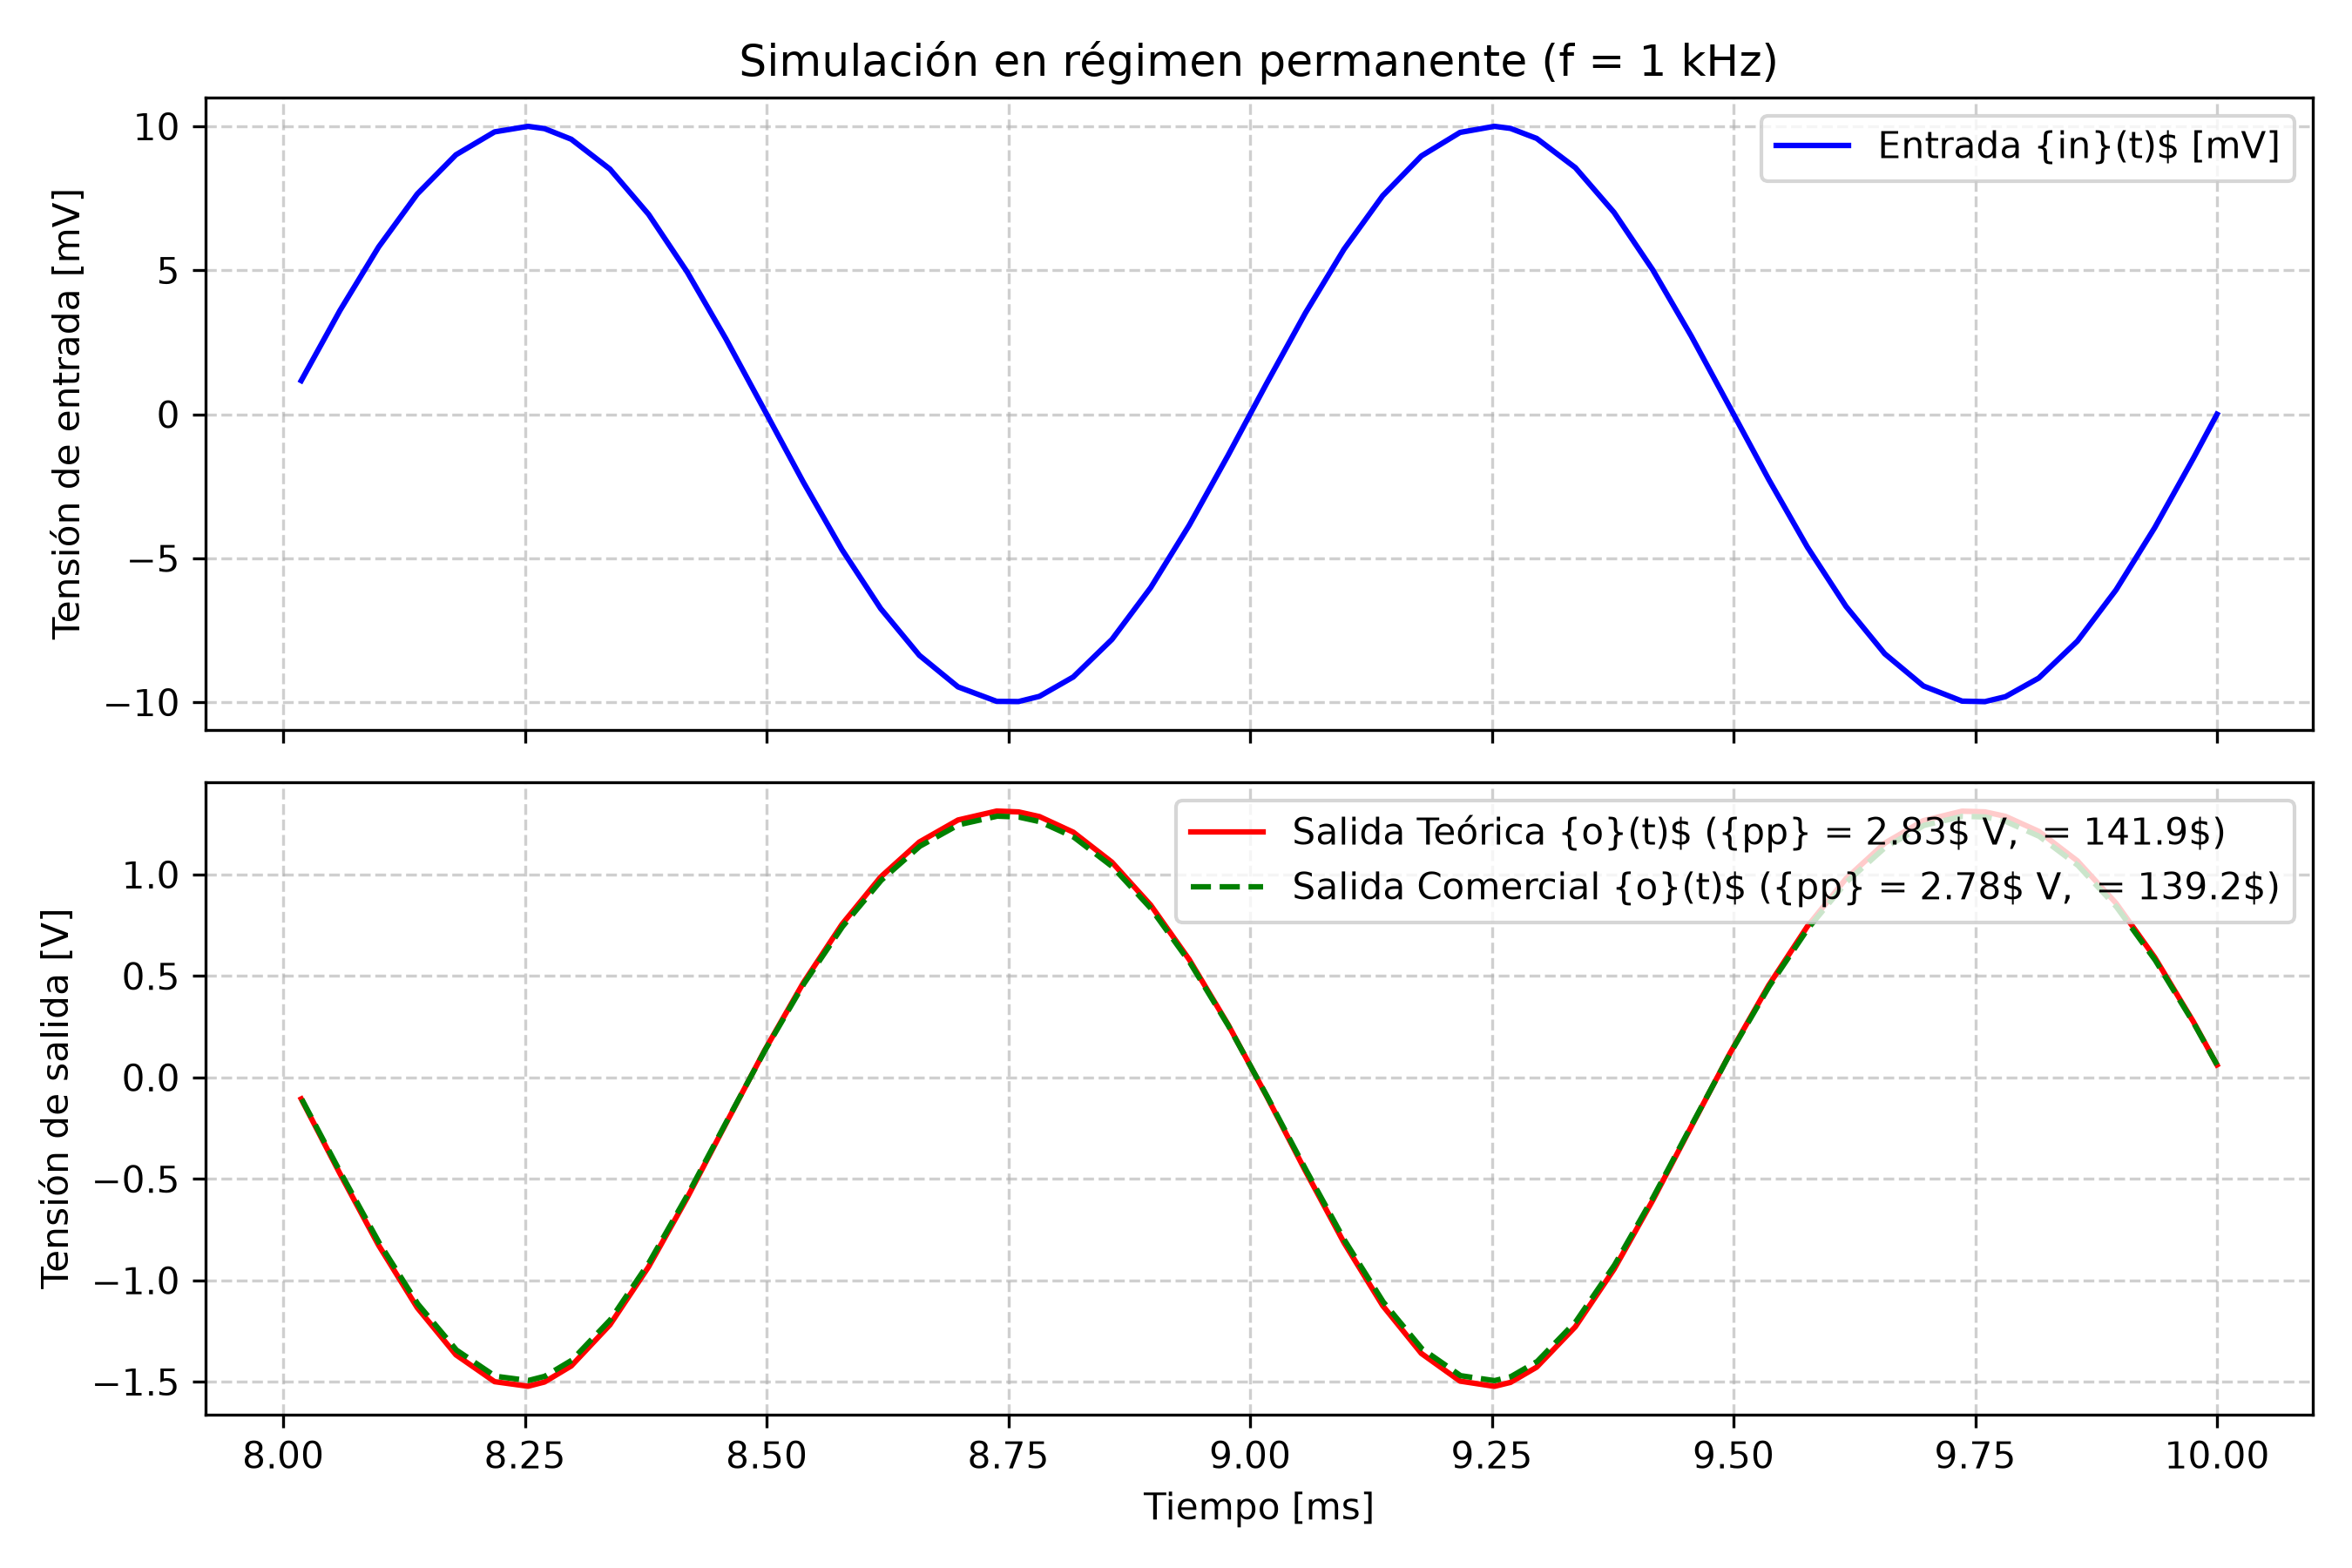
\includegraphics[width=0.92\textwidth]{images/sim_waveforms.png}
  \caption{Formas de onda en régimen permanente a $1\kHz$: comparación de tensión de entrada y salidas sobre $R_L$.}
  \label{fig:sim_waveforms}
\end{figure}

A partir de los datos crudos de simulación se constata:
\begin{itemize}
  \item Tensión de entrada pico a pico: $v_{in} = 20.00\mV_{pp}$ (amplitud de $10\mV$).
  \item Tensión de salida teórica: $v_{o,\text{teor}} = 2.8347\V_{pp}$ (mínimo $-1.5227\V$, máximo $+1.3120\V$).
    Ganancia de tensión resultante:
    \begin{equation}
      A_{v,\text{teor}} = \frac{v_{o,\text{teor}}}{v_{in}} = \frac{2.8347\V_{pp}}{0.0200\V_{pp}} \approx 141.74
    \end{equation}
  \item Tensión de salida comercial: $v_{o,\text{com}} = 2.7814\V_{pp}$ (mínimo $-1.4945\V$, máximo $+1.2869\V$).
    Ganancia de tensión resultante:
    \begin{equation}
      A_{v,\text{com}} = \frac{v_{o,\text{com}}}{v_{in}} = \frac{2.7814\V_{pp}}{0.0200\V_{pp}} \approx 139.07
    \end{equation}
\end{itemize}

La variación en la ganancia de tensión entre la etapa con valores teóricos y la normalizada es de tan solo:
\begin{equation}
  \Delta A_v = \frac{|139.07 - 141.74|}{141.74} \times 100\% \approx 1.88\%
\end{equation}
evidenciando que la sustitución por componentes comerciales no afecta de manera apreciable el desempeño amplificador
del circuito. Asimismo, en la figura~\ref{fig:sim_waveforms} se verifica con total claridad el desfase de $180^\circ$
inherente a la etapa en emisor común (inversión de fase entre base y colector).
